\chapter{Intra-Procedural Dependence Analysis}
\label{ch:dep}
Recall from Section~\ref{ch:back}.2 that two statements \ttf{S} and \ttf{T} are said to be 
dependent on each other if (a)there exists an execution path from 
\ttf{S} to \ttf{T} and (b)both statements access 
same data. As input dependence does not put any constraint on parallelization, 
our analysis takes into account the other types of dependences like flow, anti and output dependences. 
Here we redefine the general definition of data dependence in the context of heap. 
\begin{mydef}{
Two statements \ttf{S} and \ttf{T} are said to heap dependent on each 
other if (a) there exists an execution path from 
\ttf{S} to \ttf{T} and (b)both statements access 
same heap location and (c)at least one of the statements writes 
to that location.
}
\end{mydef}
We have developed a novel technique which finds out heap induced
dependencies, between any two statements in the program. The
novelty of our approach lies in the separation of shape
analysis phase from the dependence detection phase and the workflow of 
our dependence detection technique.
Our intend is to identify dependences present in the program 
following the algorithms outlined in this chapter.
Note that, our algorithms only deal with normalized statements (refer to Section~\ref{ch:back}.1), having single 
level of pointer dereference.  

In brief, our analysis works as follows: for each heap accessing statement 
in the program, our approach computes set of states i,e., set of symbolic 
locations potentially accessed by the variables in the statement and then it 
computes sets of locations which is read or written by each statement. These 
sets are then tested to identify dependences. This dependence analysis technique 
identifies memory locations in terms of abstract access paths. The abstraction 
scheme has been designed to reach the fixed-point for our algorithm. The 
details of such abstraction scheme are given next. Section~\ref{sec:depframework} gives 
overall algorithms of our analysis with details and presents the working of our algorithms with an example. 
%
\section{Access Path Abstraction}
\label{sec:accesspath}
An access path is either a symbolic location $l_0$ or location followed by a 
sequence of one or more pointer field names like $l_0\rightarrow f_1 \rightarrow 
f_2\rightarrow ...\rightarrow f_k$.  
%%In the access path symbolic location $l_0$ is referred as \emph{handle location}. 
Since an 
access path represents a path in a memory graph, it can be 
used to identify a heap node. It is hard to handle full 
length access path and the termination of the analysis becomes impossible. Hence 
we limit the length of access path to length k i,e., maximum k level of indirection 
is allowed for dereferencing. A special summary field `*' is used to limit the 
access paths, which stands for any field dereferenced beyond length k.
\begin{example}{\rm
For k = 1, all the access paths in the set $\{\loc\rightarrow\tnext\rightarrow\tnext,
  \loc\rightarrow\tnext\rightarrow\tnext\rightarrow\tnext,
  \loc\rightarrow\tnext\rightarrow\tnext
    \rightarrow\tnext\cdots\rightarrow\tnext\}$ can be abstracted as single summarized path \loc$\rightarrow$\tnext$\rightarrow{*}$. 
    Similarly assuming a data structure has two reference fields
  \lt\ and \rt, the summarized path
  $\loc\rightarrow\lt\rightarrow\rt\rightarrow{*}$ could
  stand for any of the access paths
  $\loc\rightarrow\lt\rightarrow\rt\rightarrow\lt,\ \loc\rightarrow\lt\rightarrow\rt\rightarrow\rt,\ \loc\rightarrow\lt\rightarrow\rt\rightarrow\lt\rightarrow\lt,\ \loc\rightarrow\lt\rightarrow\rt\rightarrow\lt\rightarrow\rt$
  and more such paths.
}
\hfill\psframebox{}  \end{example}
%
\section{Dependence Detection Framework} 
\label{sec:depframework}
Our method investigates if there is any heap dependency between any two statements 
in the program and the type of the dependencies following the algorithm {\tt analyze} that 
we have outlined in Figure~\ref{fig:algoTopLevel}. The algorithm  works on each function 
separately resulting in intra-procedural analysis. It takes as parameter the function to be analysed  
and the maximum length of access path, which has been set at prior. 
\begin{figure}
%\hrule
\begin{framed}
{\tt
  \begin{program}{0}
  \FL fun analyze(f, k)  \{
%  \UNL{0} CFG[f] = (N, E, Entry, Exit); \COMMENT {Control flow graph of function f}
  \UNL{0} InitSet = initialize(); \COMMENT{Initialize parameters and
  globals}
  \UNL{0} $\forall$ stmt $S_i \in$ HeapStmt[f]
  \UNL{1} tagStmt($S_i$, tagDir(UsePtrSet, DefPtrSet, AccType, Accfield));
  \UNL{0} HeapState = stateAnalysis(CFG[f]:(N, E, Entry, Exit), k);
  \UNL{0} ReadWriteSet = computeReadWrite(HeapState);
  \UNL{0} detectDependence(ReadWriteSet);
  \UNL{-1} \}
  \end{program}
}
\end{framed}
%\hrule
  Algorithm to analyze a function {\tt f} for
    dependence detection. Parameter {\tt k} is used for
    limiting the length of access paths, to keep the analysis
    bounded. 
\caption{ Intra-procedural dep. detection for a function    
    \label{fig:algoTopLevel}}
%\hrule  
\end{figure}
Summarizing, the algorithm can be divided into the following steps:

All global variables and parameters of the function under analysis are initialized 
with proper values such that the correctness of the function is not violated. As our technique
looks at only heap related statements, initialization of only global variables and parameters accessing heap 
is sufficient. The function {\tt initialize} returns {\tt InitSet}, a set of {\tt <heap directed pointer variable, symbolic location>} pairs after initialization. The symbolic locations are identified in terms of access paths as described earlier. For reasons of efficiency, length of access paths are limited to 1.

Each statement in the function is annotated with a tagging directive {\tt tagDir}. 
%The {\tt tagDir} directive is defined as {\tt tagDir(UsePtrSet, DefPtrSet, AccType, AccField)}. 
It consists of four attributes which give information regarding 
the heap accessing statement $\ttf{S_i}$ : (a)Used pointer set {\tt UsePtrSet} 
is the set of heap directed pointer variables which are used in the 
statement $\ttf{S_i}$; (b)Defined pointer set \ttf{DefPtrSet} is the set of pointer variables 
defined by the statement $\ttf{S_i}$; (c)Access type {\tt AccType} identifies 
the pattern of heap access by statement $\ttf{S_i}$ which can be categorized into following six 
classes (refer to Section~\ref{ch:back}.1).
\begin{itemize}
\item {\tt AliasStmt} : aliasing statement.
\item {\tt LinkTraverseStmt} : link traversing statement.
\item {\tt ReadStmt} : statement reading heap. 
\item {\tt WriteStmt} : statement writing into heap. 
\item {\tt FunCallStmt} : function call statement. 
\item {\tt OtherStmt} : any other statement.
\end{itemize}
(d) The access field {\tt AccField} is the pointer field accessed by the statement $\ttf{S_i}$. Table~\ref{fig:tableTagDir}  
shows example statements and corresponding tagging directives. 

\begin{table}
\centering
\begin{tabular}{| l | c |}
\hline 
\bf{Statement} & \bf{Annotation directive} \tn
\hline \hline
{\tt p = q} & {\tt tagDir(\{q\}, p, AliasStmt, null)}\\
{\tt p = q$\rightarrow$next} & {\tt tagDir(\{q\}, p, LinkTraverseStmt, next)}\tn
{\tt $\cdots$ = p$\rightarrow$data} & {\tt tagDir(\{p\}, null, ReadStmt, null)}\tn
{\tt p$\rightarrow$data = $\cdots$} & {\tt tagDir(\{p\}, null, WriteStmt, null)}\tn
%{\tt fun(p, q)} & {\tt tagDir(\{p, q\}, null, FunCallStmt, null)}\tn
\hline
\end{tabular}
\caption{Example showing different tagging directives} 
\label{fig:tableTagDir}
%\hrule
\end{table}
%%%%%%%%%%%%%%%%%%%%%%%%%%%%%%%%%%%%%%%%%%%%
\subsection{State Analysis}
This subsection introduces state analysis for heap directed variable. State analysis for heap variable involves computing a safe approximation of 
the binding of pointer variable to a set of symbolic memory locations that can be potentially accessed by the variable at a particular program point. This binding is referred as state of the variable and is represented as <\emph{variable}, \{\emph{set of symbolic locations}\}>. This analysis is essentially used by dependence analysis in future. 
\begin{mydef}{
The state of variable {\tt x} at a program point {\tt u} is the set of symbolic memory locations such that some paths from the {\tt Entry} point to {\tt u} result in the access of symbolic locations by the variable \ttf{x}.
}
\end{mydef}

The analysis works on multiple symbolic execution of the function. 
It follows general data flow analysis algorithm described in literature~\cite{Kam76globaldata, Muchnick97, Cooper02, Khedker09} etc.
It involves the following steps: (a) computation of local information, set of states after symbolic execution of each statement. At 
each program point it produces a set of states such that it contains all local and global 
variables and conservative approximation of symbolic locations accessed by each variable in the set. 
(b) computation of global information, set of possible states just before and after the execution of a block of statements. 
The control of the analysis flows in forward direction. Equations for state analysis follow the traditional data flow form: 
\begin{equation}
\ttf{In[B] = \bigcup_{P\in pred[B]}Out[P]}
\end{equation}
\begin{equation}
\ttf{Out[B] = f_B(In[B])},\   \mbox{$\ttf{f_B}$ is {\bf block level} transfer function of \ttf{B}}
\end{equation}
\begin{equation}
\ttf{f_B(In[B]) = g_{S_k}(\cdots(g_{S_1}(In[B])))},\   \mbox{$\ttf{g_{S_1}\cdots{g_{S_k}}}$ are {\bf statement level} transfer functions}
\end{equation}
Transfer function $\ttf{f_B}$ is a composition of series of 
transfer function $\ttf{g_S}$ applied to each statement present 
in the block. The first statement \ttf{S} of block \ttf{B} has 
\ttf{In} set same as the \ttf{In} set to the block. Each statement 
locally generates \ttf{Kill} and \ttf{Gen} sets which are used by 
function $\ttf{g_S}$ to produce \ttf{Out} set for each statement. 
Table~\ref{fig:genKill} shows the local effects of the statements 
handled by our analysis. Hence the statement level equations for state analysis are:
\begin{equation}
\ttf{Out[S_i] = g_{S_i}(In[S_i])},\  \mbox{\ttf{In} and \ttf{Out} sets for statement $\ttf{S_i}$}
\end{equation}
\begin{equation}
\ttf{g_{S_i}(In[S_i]) = (In[S_i]-Kill[S_i])\cup Gen[S_i]},\  \mbox{\ttf{Gen} and \ttf{Kill} are local to $\ttf{S_i}$}
\end{equation}
Figure~\ref{fig:trans} demonstrates both block level and statement 
level transfer functions. As statement \ttf{S} is the first 
statement in the basic block \ttf{B} \ttf{In[S]} has been 
set to \ttf{In[B]}. Again \ttf{Out[B]} will be 
\ttf{Out[T]} as \ttf{T} is the last statement in the block \ttf{B}. 

\begin{figure}
  \centering
  \begin{minipage}[b]{6 cm}
    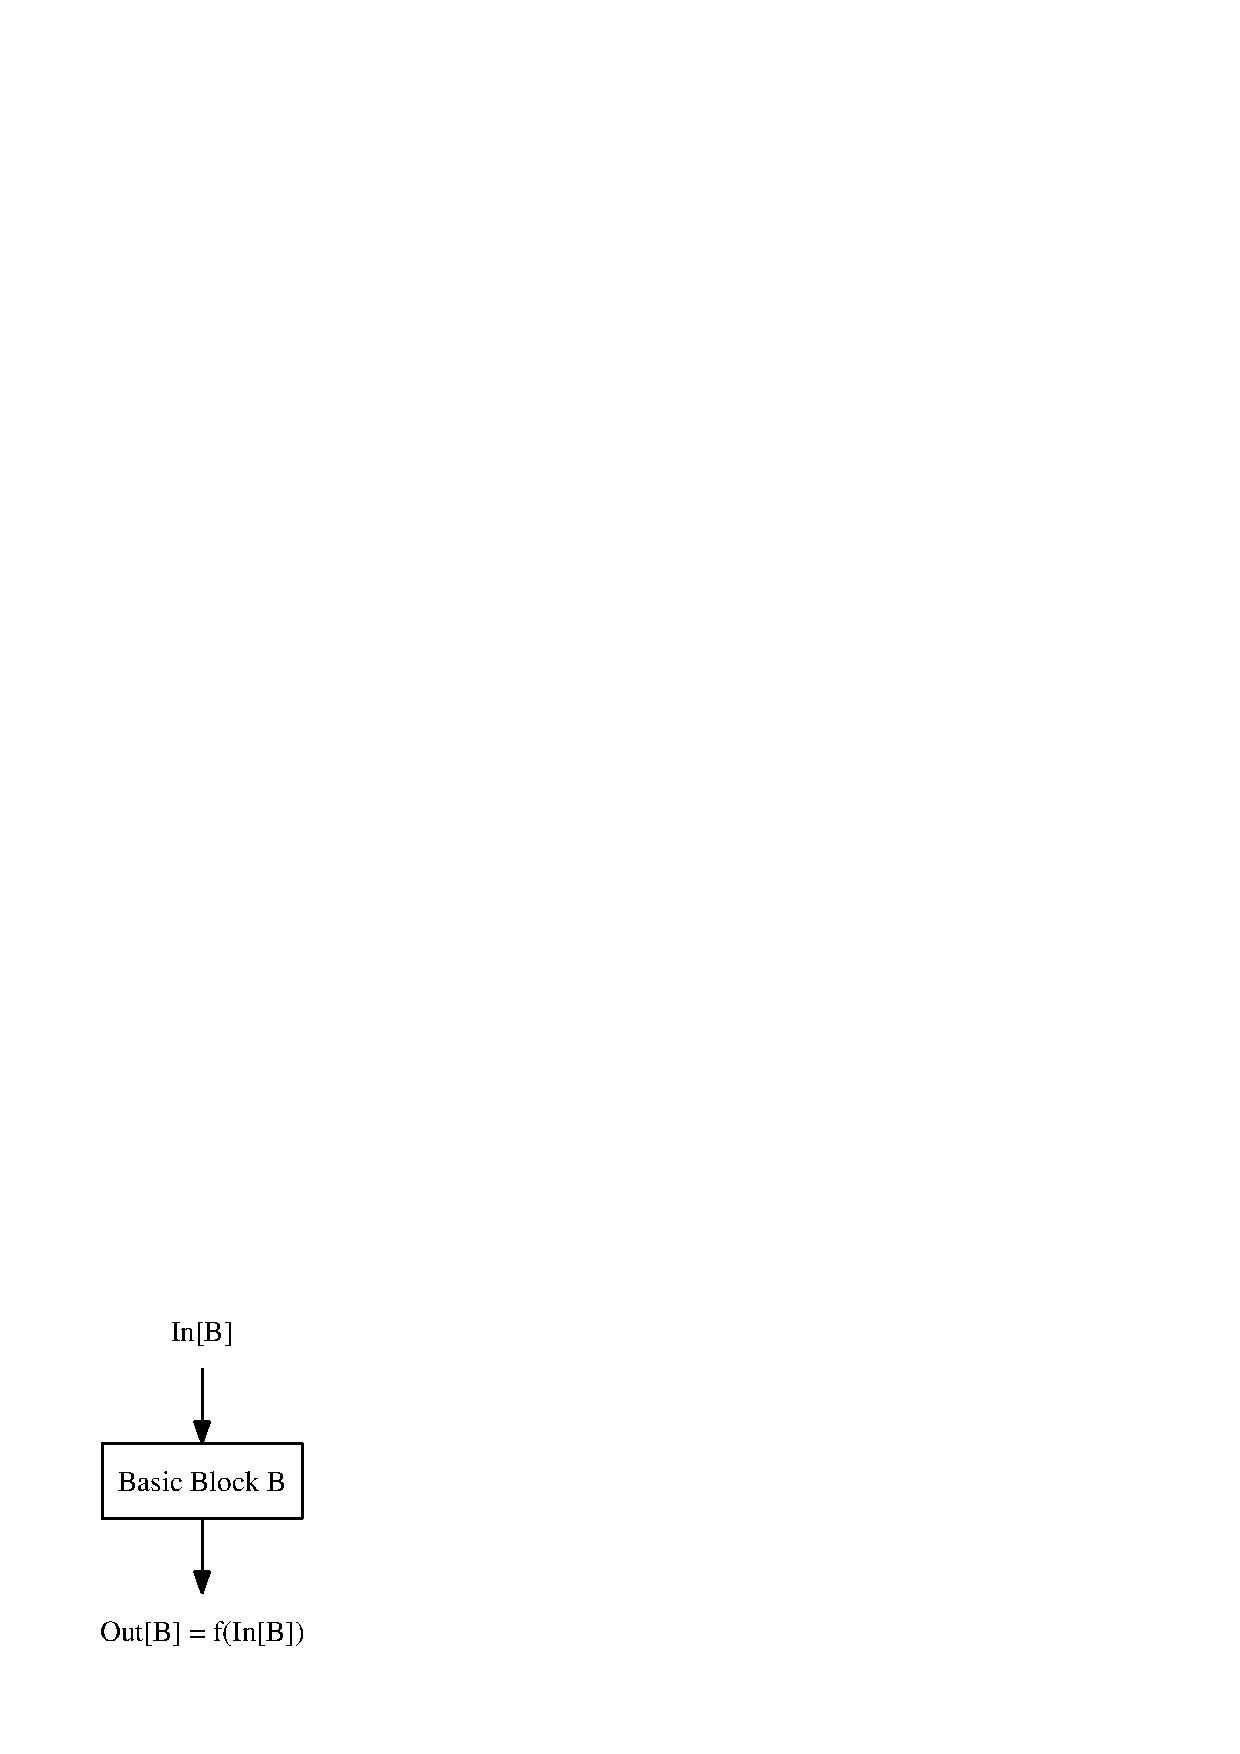
\includegraphics{grph2_text} 
    \label{labelname 1}
  \end{minipage}
  \begin{minipage}[b]{6 cm}
    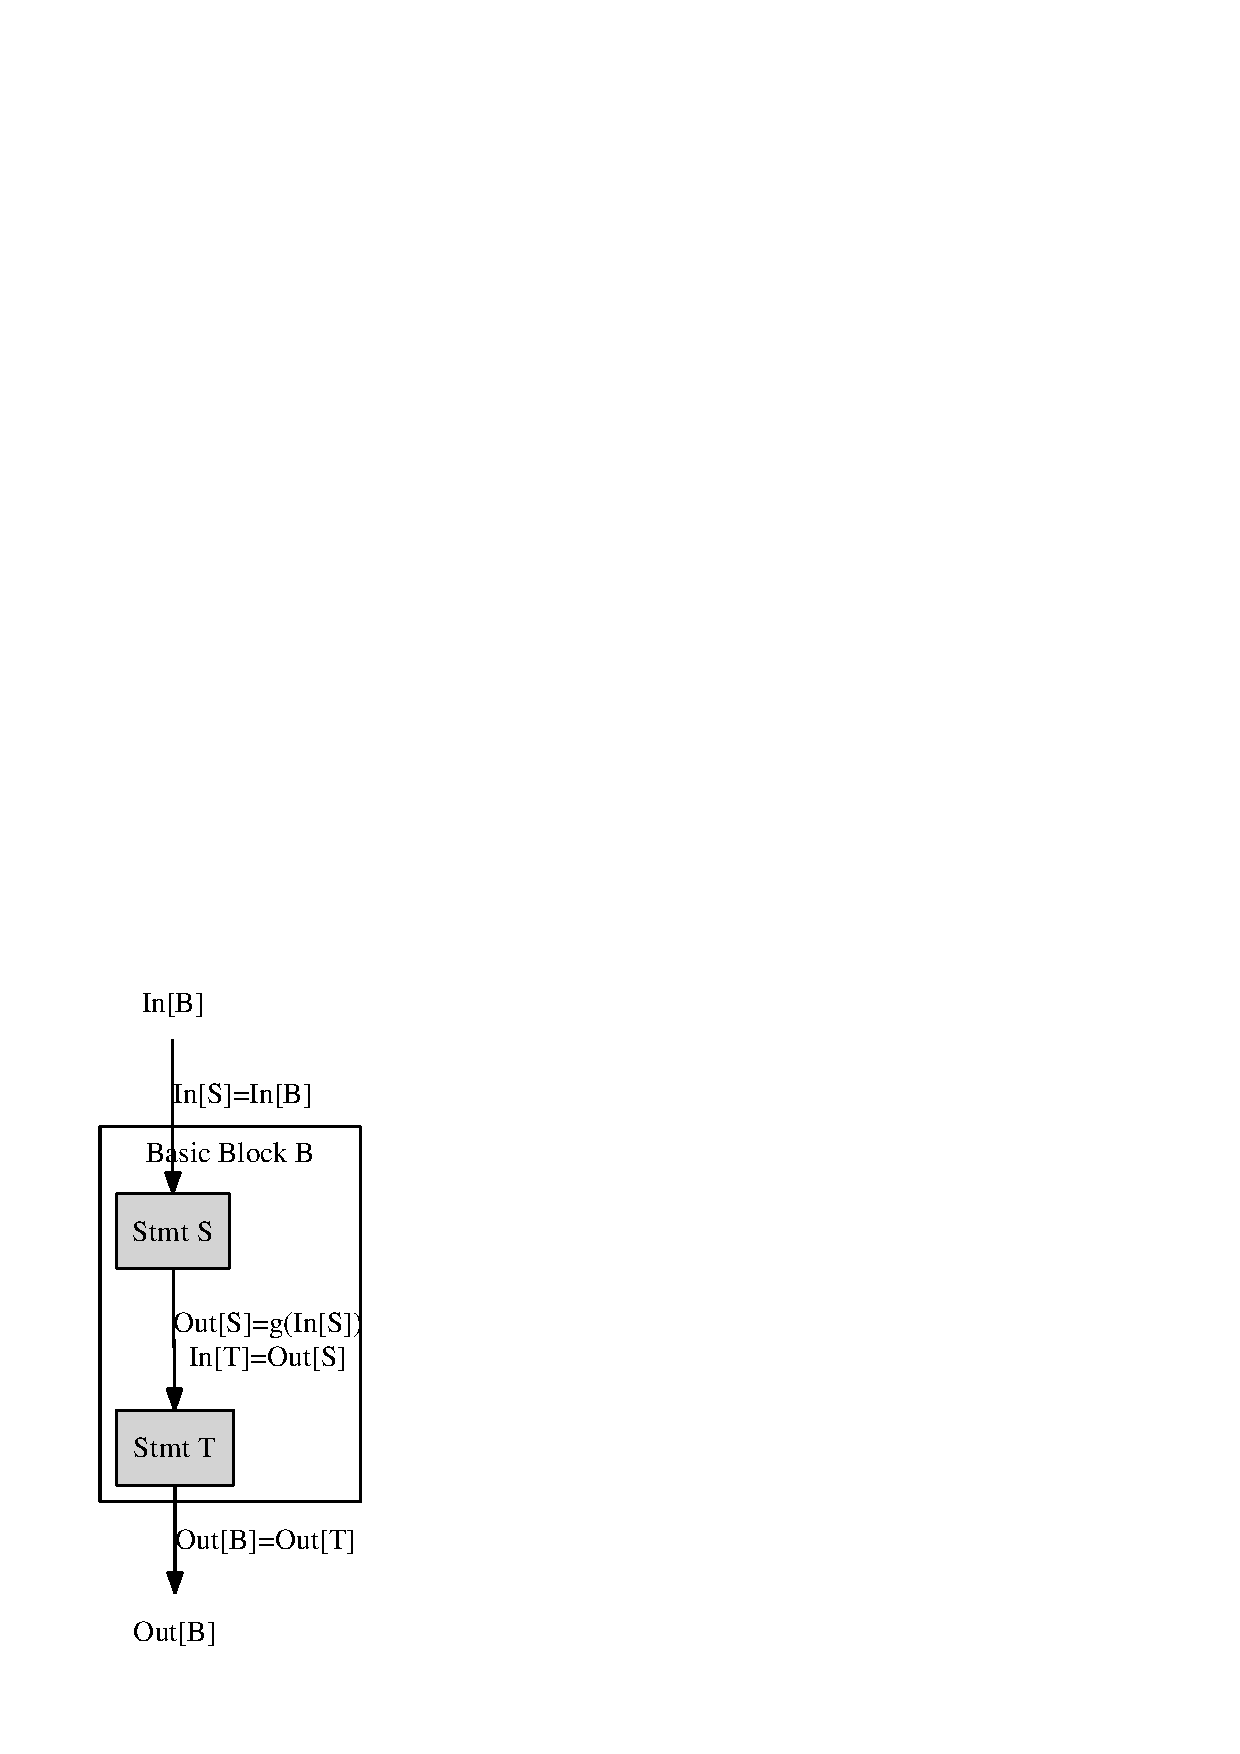
\includegraphics{grph3_text}  
%    \caption{caption 2}
    \label{labelname 2}
  \end{minipage}
  \caption{Transfer function for basic block}
   \label{fig:trans}
\end{figure}
%%%%%%%%%%%%%%%%%%%%%%%%%%%%%%%%%%%%
\begin{table}
\centering
\begin{tabular}{| l | c | c |}
\hline 
Statement & Gen set & Kill set \tn
\hline \hline
1. {\tt p = q} & {\tt \{<p,m> | <q,m>$\in$In[S]\}} & {\tt \{<p,l> | <p,l>$\in$In[S]\}} \tn
2. {\tt p = q\rtarrow next} & {\tt \{<p,m\rtarrow next> | <q,m>$\in$In[S]\}} & {\tt \{<p,l> | <p,l>$\in$In[S]\}} \tn
3. {\tt $\cdots$ = p\rtarrow data} & $\phi$ & $\phi$ \tn
4. {\tt p$\rightarrow$data = $\cdots$} & $\phi$ & $\phi$ \tn
5. {\tt fun(p, q)} & $\phi$ & $\phi$ \tn
\hline
\end{tabular}
\caption{\emph{Gen} and \emph{Kill} set for each statement} 
\label{fig:genKill}
%\hrule
\end{table}

The overall algorithm for state analysis is outlined in Figure~\ref{fig:AlgoStateAnal}. 
\ttf{Out[Entry]} is initialized to {\tt InitSet} to set the boundary condition. 
The \emph{while} loop in the algorithm iterates until it reaches the fixed-point. 
{\tt stateTrans} gives the algorithm for transfer function which works on each block. 
Though {\tt Gen} and {\tt Kill} informations are local to each statement they are 
computed in each iteration of the analysis, conflicting general data flow analysis algorithm. 
 
%%%%%%%%%%%%%%%%%%%%%%%%%%%%%%%%%%%%%%%%%%
\begin{figure}
%\hrule
\begin{framed}
{\tt
  \begin{program}{0}
  \FL fun stateAnalysis(CFG[f]:(N, E, Entry, Exit), k)  \{
  \UNL{0} Out[Entry] = InitSet; \COMMENT{Boundary condition}
  \UNL{0} \FOR each basic block B other than Entry
  \UNL{0} \COMMENT{Initialization for iterative algorithm}
  \UNL{1} Out[B] = $\phi$; 
  \UNL{0} \WHILE{(changes to any Out[ ] occur)} \{ \COMMENT{Iterate}
  \UNL{1} \FOR each basic block B other than Entry \{
  \UNL{2} In[B] = $\bigcup$(Out[P]), for all predecessors P of B;
  \UNL{2} Out[B] = stateTrans(B, In[B], k);
  \UNL{1} \}
  \UNL{0} \}
  \UNL{-1} \}
  \end{program}
}
\end{framed}
%\hrule
  \caption{Algorithm defining state analysis. \label{fig:AlgoStateAnal}}
%\hrule  
\end{figure}
%%%%%%%%%%%%%%%%%%%%%%%%%%%%%%%%%%%%%%%%%%%%%%%%%
\begin{figure}
%\hrule
\begin{framed}
{\tt
  \begin{program}{0}
  \FL fun stateTrans(Basic Block:BB, In set of BB:In[BB], k)  \{
  \UNL{0} TempState = In[BB];
  \UNL{0} \FOR each Stmt $S_i\in$ HeapStmt[BB] \{ \COMMENT{HeapStmt[BB] contains}
  \UNL{0} \COMMENT {heap intensive statements of BB}
  \UNL{1} In[$S_i$] = TempState;
  \UNL{1} Kill[$S_i$] = findStateDefVar(TempState, $S_i$);
  \UNL{1} Gen[$S_i$] = computeState(In[$S_i$], $S_i$);
%  \UNL{1} OldOut[$S_i$] = Out[$S_i$];
  \UNL{1} Out[$S_i$] = (In[$S_i$] - Kill[$S_i$]) $\cup$ Gen[$S_i$];
  \UNL{1} tempState = Out[$S_i$];
  \UNL{0} \}
  \UNL{0} return tempState;
  \UNL{-1} \}
  \end{program}
}
\end{framed}
%\hrule
  \caption{Algorithm for block level transfer function. \label{fig:AlgoGenState}}
%\hrule  
\end{figure}
%%%%%%%%%%%%%%%%%%%%%%%%%%%%%%%%%%%%
\begin{figure}
%\hrule
\begin{framed}
{\tt
  \begin{program}{0}
  \FL fun findStateDefVar(Set of States:TempState, Statement:$S_i$)  \{
  \UNL{0} Set of States : CurrState, LocalState = $\phi$;
%  \UNL{0} Set of variables used in Stmt : UseVarSet = $\phi$;
%  \UNL{0} UseVarSet = findUseVar(Stmt);\COMMENT{Detects variables used in Stmt}
  \UNL{0} \FOR each variable $V_i\in$ DefPtrSet \{
  \UNL{1} Find the state {\tt CurrState} of $V_i$ from {\tt TempState};
 \UNL{1} LocalState = LocalState $\cup$ CurrState;
  \UNL{0} \}
  \UNL{0} return LocalState;
  \UNL{-1} \}
  \end{program}
}
\end{framed}
%\hrule
  \caption{Computing \emph{Kill} set.\label{fig:AlgoFindStateDefVar}}
%\hrule  
\end{figure}
%%%%%%%%%%%%%%%%%%%%%%%%%%%%%%%%%%%%%%%%%%%%%%
\begin{figure}
%\hrule
\begin{framed}
{\tt
  \begin{program}{0}
  \FL fun computeState(In set of stmt:In[Stmt], Statement:Stmt)  \{
  \UNL{0} UseVarSet = findStateUseVar(In[Stmt], Stmt);
  \UNL{0} if Stmt $\equiv$ p = q 
  \UNL{1} Gen[Stmt] = \{ <p,$l_0$> | <q,$l_0$> $\in$ UseVarSet \} 
  \UNL{3} $\vee$ \{ <p,$l_0\rightarrow$sel> | <q,$l_0\rightarrow$sel> $\in$ UseVarSet \}
  \UNL{3} $\vee$ \{ <p,$l_0\rightarrow$sel$\rightarrow$*> | <q,$l_0\rightarrow$sel$\rightarrow$*> $\in$ UseVarSet \};
  \UNL{0} else if Stmt $\equiv$ p = q$\rightarrow$next
  \UNL{1} Gen[Stmt] = \{ <p,$l_0\rightarrow$next> | <q,$l_0$> $\in$ UseVarSet \} 
  \UNL{3} $\vee$ \{ <p,$l_0\rightarrow$sel$\rightarrow$*> | <q,$l_0\rightarrow$sel> $\in$ UseVarSet \};
  \UNL{0} else if Stmt $\equiv$ $\cdots$ = p$\rightarrow$data
  \UNL{1} Gen[Stmt] = In[Stmt];
  \UNL{0} else if Stmt $\equiv$ p$\rightarrow$data = $\cdots$
  \UNL{1} Gen[Stmt] = In[Stmt];
  \UNL{0} else if Stmt $\equiv$ f(p,q)
  \UNL{1} Gen[Stmt] = In[Stmt];
  \UNL{0} else Gen[Stmt] = $\phi$;
  \UNL{-1} \}
  \end{program}
}
\end{framed}
%\hrule
  \caption{Computing \emph{Gen} set. \label{fig:AlgoComputeState}}
%\hrule  
\end{figure}
%%%%%%%%%%%%%%%%%%%%%%%%%%%%%%%%%%%%%%%%%%
\begin{figure}
%\hrule
\begin{framed}
{\tt
  \begin{program}{0}
  \FL fun findStateUseVar(Set of States:TempState, Statement:$S_i$)  \{
  \UNL{0} Set of States : CurrState, LocalState = $\phi$;
%  \UNL{0} Set of variables used in Stmt : UseVarSet = $\phi$;
%  \UNL{0} UseVarSet = findUseVar(Stmt);\COMMENT{Detects variables used in Stmt}
  \UNL{0} \FOR each variable $V_i\in$ UsePtrSet \{
  \UNL{1} Find the state {\tt CurrState} of $V_i$ from {\tt TempState};
  \UNL{1} LocalState = LocalState $\cup$ CurrState;
  \UNL{0} \}
  \UNL{0} return LocalState;
  \UNL{-1} \}
  \end{program}
}
\end{framed}
%\hrule
  \caption{Computing states of used variables. \label{fig:AlgoFindStateUseVar}}
%\hrule  
\end{figure}
\begin{example}{\rm
We illustrate via an example the way our algorithm works. Let's consider the code fragment shown in Figure~\ref{ch:Intro}.2(b). 
Global variables and parameters of the code are initialized to {\tt InitSet} consisting of \ttf{\{<list, $l_0$>\}}. Table~\ref{fig:tableState} 
shows the set of states produced by each statement in the code and demonstrates how the analysis reaches fixed-point. 
Note that the length of access path is limited to 1. In this example \ttf{Out} set for each basic block in iteration number 2 is same as \ttf{Out} set produced by each block in iteration number 3. Hence in third iteration the algorithm reaches fixed-point.
}
\hfill\psframebox{}  \end{example}

\begin{table}
\centering
\begin{tabular}{| l | c | c |}
\hline 
Statement & Iteration 1 & Iteration 2 \tn
\hline \hline
S1: {\tt p = list} & {\tt In = \{<list,$l_0$>\}} & {\tt In = \{<list,$l_0$>\}} \tn %\cline{1-1}
& {\tt Gen = \{<p,$l_0$>\}} & {\tt Gen = \{<p,$l_0$>\}} \tn
& {\tt Kill = \{$\phi$\}} & {\tt Kill = \{$\phi$\}} \tn
& {\tt Out = \{<list,$l_0$>,<p,$l_0$>\}} & {\tt Out = \{<list,$l_0$>,<p,$l_0$>\}} \tn 
\hline
{\tt while() \{} & {\tt In = \{<list,$l_0$>,<p,$l_0$>\}} & {\tt In = \{<list,$l_0$>,<p,$l_0$>,} \tn %\cline{1-1}
& & {\tt <p,$l_0\rightarrow$next$\rightarrow${*}>,} \tn
& & {\tt <q,$l_0\rightarrow$next>,}\tn
& & {\tt <r,$l_0\rightarrow$next$\rightarrow${*}>\} = C}(say) \tn
%& & {\tt = C(say)} \tn
& {\tt Out = \{<list,$l_0$>,<p,$l_0$>\}} & {\tt Out = C} \tn
\hline
S2: {\tt q = p$\rightarrow$next} & {\tt In = \{<list,$l_0$>,<p,$l_0$>\}} & {\tt In = C} \tn %\cline{1-1}
& {\tt Gen = \{<q,$l_0\rightarrow$next>\}} & {\tt Gen = \{<q,$l_0\rightarrow$next>,} \tn
& & {\tt <q,$l_0\rightarrow$next$\rightarrow${*}>\}} \tn
& {\tt Kill = $\phi$} & {\tt Kill = \{<q,$l_0\rightarrow$next>\}} \tn
& {\tt Out = \{<list,$l_0$>,<p,$l_0$>,} & {\tt Out = \{C,<q,$l_0\rightarrow$next$\rightarrow${*}\}} \tn
& {\tt <q,$l_0\rightarrow$next>\} = A}(say)&  {\tt = D}(say) \tn
%& {\tt = A(say)}& {\tt = D(say)} \tn
\hline
S3: {\tt temp = q$\rightarrow$num} & {\tt In = A} & {\tt In = D} \tn
& {\tt Out = A} & {\tt Out = D} \tn
\hline
S4: {\tt r = q$\rightarrow$next} & {\tt In = A} & {\tt In = D} \tn
& {\tt Gen = \{<r,$l_0\rightarrow$next$\rightarrow${*}>\}} & {\tt Gen = \{<r,$l_0\rightarrow$next$\rightarrow${*}>\}} \tn
& {\tt Kill = $\phi$} & {\tt Kill = \{<r,$l_0\rightarrow$next$\rightarrow${*}>\}} \tn
& {\tt Out = \{A,<r,$l_0\rightarrow$next$\rightarrow${*}>\}} & {\tt Out = D} \tn
%& {\tt <r,$l_0\rightarrow$next$\rightarrow${*}>\}} & \tn
& {\tt = B}(say) & \tn
\hline
S5: {\tt r$\rightarrow$num = temp} & {\tt In = B} & {\tt In = D} \tn
& {\tt Out = B} & {\tt Out = D} \tn
\hline
S6: {\tt p = r} & {\tt In = B} & {\tt In = D} \tn
& {\tt Gen = \{<p,$l_0\rightarrow$next$\rightarrow${*}>\}} & {\tt Gen = \{<p,$l_0\rightarrow$next$\rightarrow${*}>\}} \tn
& {\tt Kill = \{<p,$l_0$>\}} &{\tt Kill = \{<p,$l_0$>,} \tn
& & {\tt <p,$l_0\rightarrow$next$\rightarrow${*}>\}} \tn
& {\tt Out = \{<list,$l_0$>,} & {\tt Out = \{<list,$l_0$>,} \tn
& {\tt <p,$l_0\rightarrow$next$\rightarrow${*}>,} & {\tt <p,$l_0\rightarrow$next$\rightarrow${*}>,} \tn
& {\tt <q,$l_0\rightarrow$next>,} & {\tt <q,$l_0\rightarrow$next>,} \tn
& {\tt <r,$l_0\rightarrow$next$\rightarrow${*}>\}} & {\tt <q,$l_0\rightarrow$next$\rightarrow${*}>,} \tn
& & {\tt <r,$l_0\rightarrow$next$\rightarrow${*}>\}} \tn
\hline
\end{tabular}
\caption{Set of states for each statement of an example code} 
\label{fig:tableState}
%\hrule
\end{table}

%%%%%%%%%%%%%%%%%%%%%%%%%%%%%%%%%%%%%%%%%%%%%%%%%%%%s
\begin{figure}
%\hrule
\begin{framed}
{\tt
  \begin{program}{0}
  \FL fun computeReadWrite(Set of States:HeapStates)  \{
  \UNL{0} Set of States : CurrState, LocalState = $\phi$;
  \UNL{0} \FOR each stmt $S_i$ \{
  \UNL{1} \IF ($S_i$ $\equiv$ $\cdots$ = p$\rightarrow$num) \{ \COMMENT{statement reading heap}
  \UNL{2} ReadSet = findStateUseVar (HeapStates[$S_i$], $S_i$);
  \UNL{2} WriteSet = $\phi$;
  \UNL{1} \}
  \UNL{1} \IF else ($S_i$ $\equiv$ p$\rightarrow$num = $\cdots$) \{ \COMMENT{statement writing into heap}
  \UNL{2} ReadSet = $\phi$;
  \UNL{2} WriteSet = findStateUseVar (HeapStates[$S_i$], $S_i$);
  \UNL{1} \}
  \UNL{1} \IF else ($S_i$ $\equiv$ f(p,q)) \{ \COMMENT{function call statement}
  \UNL{2} ReadSet = findStateUseVar (HeapStates[$S_i$], $S_i$);
  \UNL{2} WriteSet = findStateUseVar (HeapStates[$S_i$], $S_i$);
  \UNL{1} \}
  \UNL{1} else \{
  \UNL{2} ReadSet = $\phi$;
  \UNL{2} WriteSet = $\phi$;
  \UNL{1} \}
  \UNL{0} \}
  \UNL{-1} \}
  \end{program}
}
\end{framed}
%\hrule
  \caption{computing Read and Write sets. \label{fig:AlgoReadWrite}}
%\hrule  
\end{figure}
%%%%%%%%%%%%%%%%%%%%%%%%%%%%%%%%%%%%%%%%%%%%%%%%%%%%%%
\subsection{Read/Write State Computation}
For each statement we intend to compute two sets of heap access 
paths: (a)\emph{Read set}: the set of paths which are accessed 
to read a heap location and (b)\emph{Write set}: the set of paths 
which are accessed to write to a heap location. These sets are 
obtained from the set of states, generated by the state analysis, in a single 
pass over the function. The read and write sets are used 
later to identify dependences. 

Function {\tt computeReadWrite} 
referred in Figure~\ref{fig:AlgoReadWrite} computes such sets in a 
single symbolic execution of the function. 
Function {\tt findStateUseVar} is used to generate {\tt Read} 
and {\tt Write} sets for statements reading/writing heap. Function calls are handled by
conservative read/write sets that over approximate the
heap locations that could potentially be read or written
inside the called function. Read and write sets for other statements are set to $\phi$. 

 \begin{figure}[t]
  \begin{center}
  
    \scalebox{.8}{\begin{tabular}{ c | c }
%    \hline
      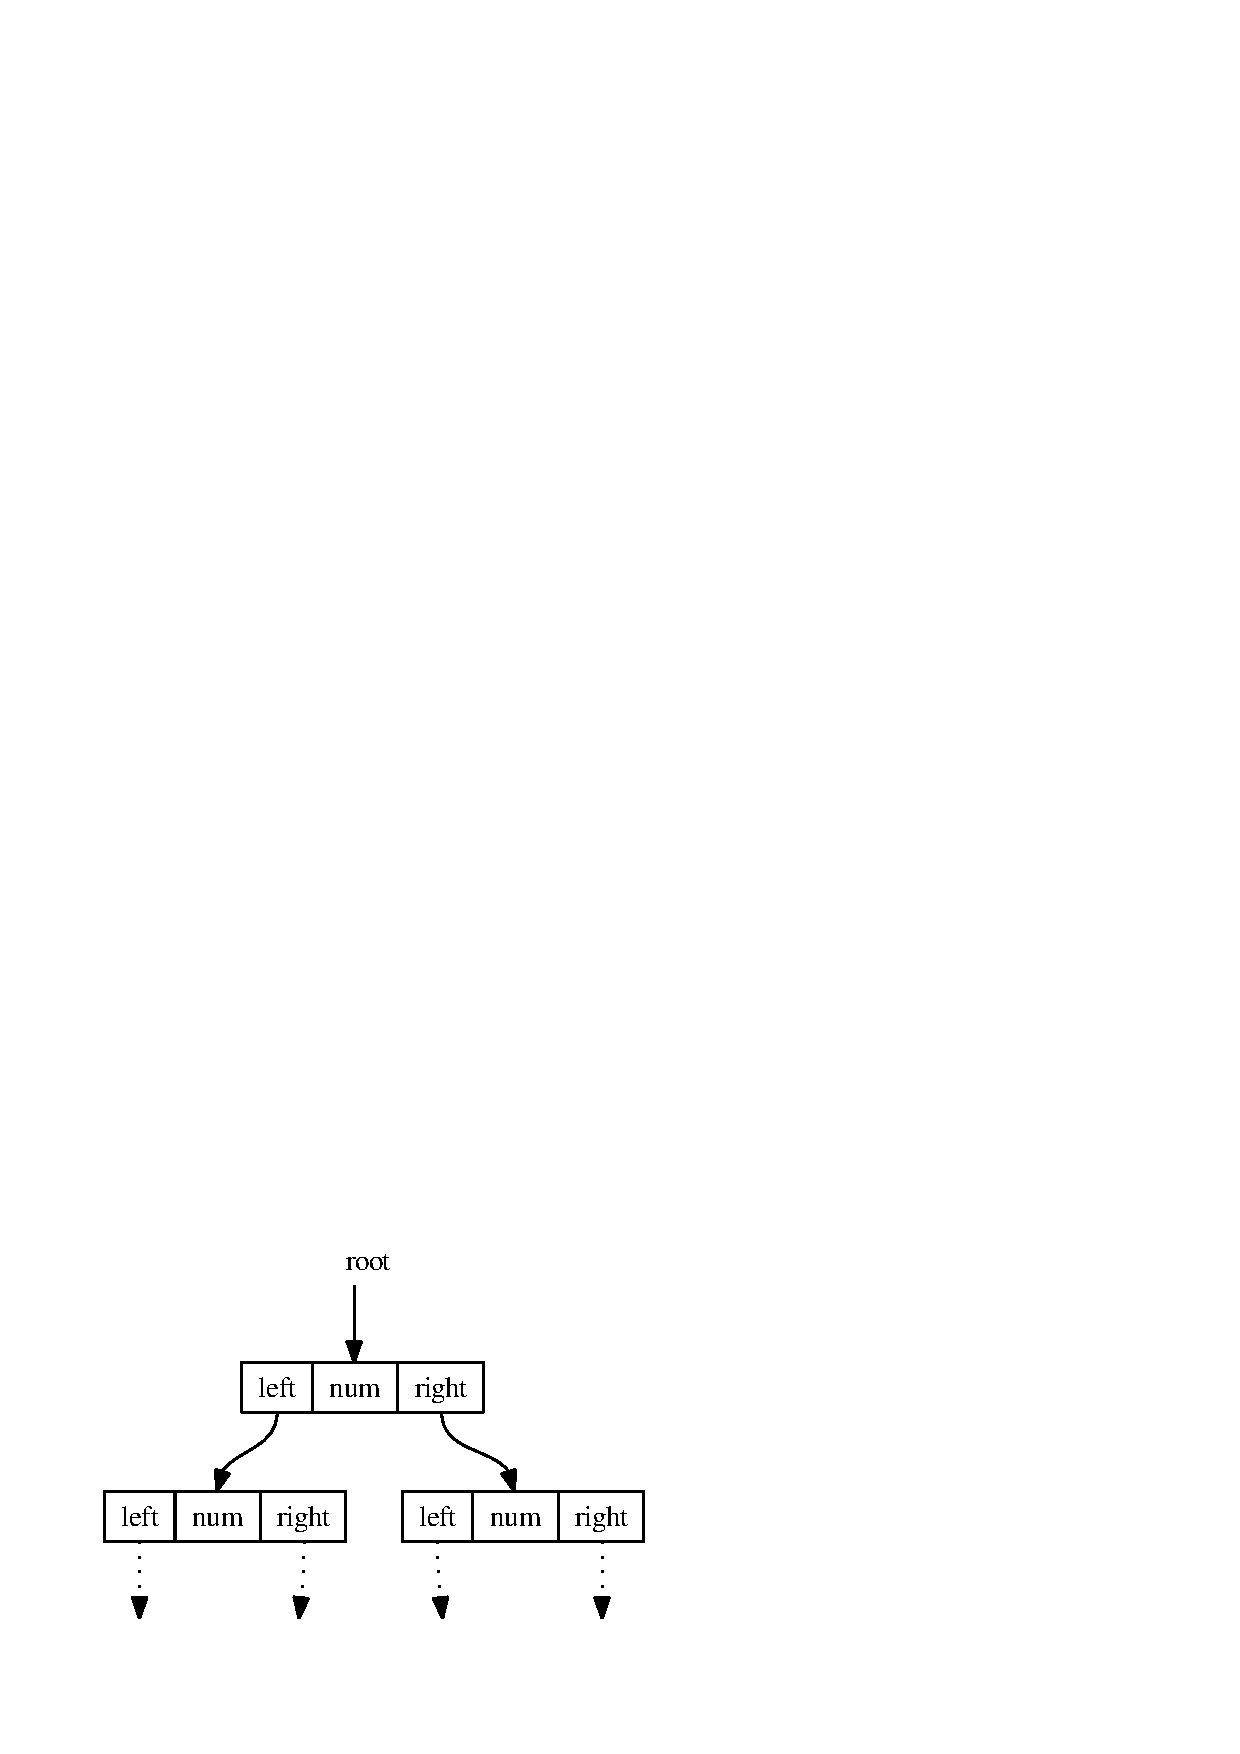
\includegraphics[scale=0.75]{tree_grph} %\cline{1-1}
      &
      {\tt
\begin{program}{10}
  \FL\ \ldots
  \NL{0} p = tree;
  \UNL{0} \WHILE (p$\rightarrow$left != NULL) \{
  \NL{1}     newFunc (p);
%  \NL{1}     temp = q$\rightarrow$num;
  \NL{1}     p = p$\rightarrow$left;
%  \NL{1}     r$\rightarrow$num = temp;
%  \NL{1}     myFunc (q, r);
%  \NL{1}     p = r;
  \UNL{0} \}
  \UNL{0} \ldots \\
 \\
 \\
 \\
 \\
  %
\end{program}
}
 \\
      (a) Tree data structure. & 
      (b) Code fragment traversing the data structure. \\
%      \hline
    \end{tabular}}
  \end{center}
  \hrule
  \caption{\label{fig:func} Program with function call.}
\end{figure}
%
\begin{example}{\rm Consider the code fragment shown in Figure~\ref{fig:func}(b) which traverses 
the Tree data structure shown in Figure~\ref{fig:func}(a). 
Our analysis conservatively approximates read and write sets for statement \ttf{S12} which is a function call statement. 
The analysis generates the read and write sets as \ttf{\{<p, $l_0$>, 
<p, $l_0$\rtarrow{*}>\}} which is the worst case approximations of such sets. 
}
\hfill\psframebox{}  \end{example}

Our approach is conservative in the sense that the read set
and write set we compute for a statement are over
approximations of the actual locations that are read or
written by the statement. Therefore it is possible that our
analysis reports two statement to be dependent when they are
not really dependent on each other. However, this can inhibit
some parallelizing optimization but can not result in an
incorrect parallelization. 
\begin{table}
\centering
\begin{tabular}{| l | c | c |}
\hline 
Statement & Read set & Write set \tn
\hline
S1: {\tt p=list} & {\tt $\phi$} & {\tt $\phi$}\tn
S2: {\tt q=p$\rightarrow$next} & {\tt $\phi$} & {\tt $\phi$} \tn
S3: {\tt temp=q$\rightarrow$num} & {\tt \{<q,$l_0\rightarrow$next>,} & {\tt $\phi$} \tn
& {\tt <q,$l_0\rightarrow$next$\rightarrow${*}>\}} & \tn
S4: {\tt r=q$\rightarrow$next} & {\tt $\phi$} & {\tt $\phi$} \tn
S5: {\tt r$\rightarrow$num=temp} & {\tt $\phi$} & {\tt \{<r,$l_0\rightarrow$next$\rightarrow${*}>\}}\tn
%S6: {\tt myFunc(p,q)} & {\tt \{<p,$l_0\rightarrow$next>,} & {\tt \{<p,$l_0\rightarrow$next>,} \tn
%& {\tt <p,$l_0\rightarrow$next$\rightarrow${*}>,} & {\tt <p,$l_0\rightarrow$next$\rightarrow${*}>} \tn
%& {\tt <q,$l_0\rightarrow$next>,} & {\tt <q,$l_0\rightarrow$next>,} \tn
%& {\tt <q,$l_0\rightarrow$next$\rightarrow${*}>\}} & {\tt <q,$l_0\rightarrow$next$\rightarrow${*}>\}} \tn
S6: {\tt p=r} & {\tt $\phi$} & {\tt $\phi$} \tn
\hline
\end{tabular}
\caption{Read and write sets accessed by each statement} 
\label{fig:tableReadWrite}
%\hrule
\end{table}
\subsection{Dependence Detection}
Our approach identify memory locations in terms of 
access paths as mentioned earlier. Multiple access 
paths can exist at a time leading to same location. 
Hence we need some method to detect whether two paths 
access same location or not. Our analysis needs to know 
if any two access paths potentially share a common heap object. 
Shape analysis as referred in~\cite{sandeep} produces an 
interface \ttf{isInterfering(p, $\alpha$, q, $\beta$)} 
to detect such interference. For heap pointers \ttf{p}, 
\ttf{q} and field sequences $\alpha, \beta, \alpha', \beta'$, 
this function returns true if the
paths {\tt p.$\alpha'$} and {\tt q.$\beta'$} interfere
(potentially reach the same heap node at run-time), and
$\alpha$ and $\beta$ are prefixes of $\alpha'$ and $\beta'$
respectively.

Read and write sets thus generated are tested to detect 
various dependences (flow, anti or output). Let \ttf{S} and \ttf{T} 
be statements in the program such that there exists an execution 
path from \ttf{S} to \ttf{T}. Then the dependence of \ttf{T} on 
\ttf{S} can be defined as follows:

\newcommand{\flowdep}{\mbox{flow-dep}}
\newcommand{\antidep}{\mbox{anti-dep}}
\newcommand{\outputdep}{\mbox{output-dep}}
\newcommand{\rs}[1]{\mbox{read}(#1)}
\newcommand{\ws}[1]{\mbox{write}(#1)}
\newcommand{\rst}[2]{\mbox{read}(#1, #2)}
\newcommand{\wst}[2]{\mbox{write}(#1, #2)}
\newcommand{\set}{\mbox{set}}
\noindent

$\begin{array}{rcl}
\interf{\set_1}{\set_2} &\equiv& \isInterfering(p, \alpha, q,
\beta) \; \mbox{where } 
p.\alpha \in \set_1   \wedge  q.\beta \in \set_2 \\ 
\flowdep(S, T) &\equiv& \interf{\ws{S}}{\rs{T}} \\ 
\antidep(S, T) &\equiv& \interf{\rs{S}}{\ws{T}} \\
\outputdep(S, T) &\equiv& \interf{\ws{S}}{\ws{T}}
\end{array}$ \\
\noindent where \isInterfering\ is the function provided by
shape analysis.

\begin{example} {\label{ex:dep}\rm
Table~\ref{fig:tableReadWrite} shows the read and write sets for each statement in
the example code of Figure~\ref{ch:Intro}.2(b). From the table,
we can infer all the dependences of which few are listed here:
\begin{enumerate}
\item loop independent anti-dependence  from statement {S3} to
statement {S5}
\item loop carried flow-dependence  from statement {S5} to
statement {S3}
\item loop independent output-dependence from statement {S5} 
to statement {S6}
\item loop carried anti-dependence from statement {S6} to statement {S5}
\end{enumerate}  
Due to presence of loop carried dependences different iterations of the loop can not be executed in parallel. Next we explain how we can further refine our dependence
analysis to filter out some spurious dependences.
}
\hfill\psframebox{}  \end{example}

